\documentclass[ignorenonframetext,]{beamer}
\setbeamertemplate{caption}[numbered]
\setbeamertemplate{caption label separator}{: }
\setbeamercolor{caption name}{fg=normal text.fg}
\beamertemplatenavigationsymbolsempty
\usepackage{lmodern}
\usepackage{amssymb,amsmath}
\usepackage{ifxetex,ifluatex}
\usepackage{fixltx2e} % provides \textsubscript
\ifnum 0\ifxetex 1\fi\ifluatex 1\fi=0 % if pdftex
\usepackage[T1]{fontenc}
\usepackage[utf8]{inputenc}
\else % if luatex or xelatex
\ifxetex
\usepackage{mathspec}
\else
\usepackage{fontspec}
\fi
\defaultfontfeatures{Ligatures=TeX,Scale=MatchLowercase}
\fi
% use upquote if available, for straight quotes in verbatim environments
\IfFileExists{upquote.sty}{\usepackage{upquote}}{}
% use microtype if available
\IfFileExists{microtype.sty}{%
\usepackage{microtype}
\UseMicrotypeSet[protrusion]{basicmath} % disable protrusion for tt fonts
}{}
\newif\ifbibliography
\usepackage{color}
\usepackage{fancyvrb}
\newcommand{\VerbBar}{|}
\newcommand{\VERB}{\Verb[commandchars=\\\{\}]}
\DefineVerbatimEnvironment{Highlighting}{Verbatim}{commandchars=\\\{\}}
% Add ',fontsize=\small' for more characters per line
\usepackage{framed}
\definecolor{shadecolor}{RGB}{248,248,248}
\newenvironment{Shaded}{\begin{snugshade}}{\end{snugshade}}
\newcommand{\KeywordTok}[1]{\textcolor[rgb]{0.13,0.29,0.53}{\textbf{{#1}}}}
\newcommand{\DataTypeTok}[1]{\textcolor[rgb]{0.13,0.29,0.53}{{#1}}}
\newcommand{\DecValTok}[1]{\textcolor[rgb]{0.00,0.00,0.81}{{#1}}}
\newcommand{\BaseNTok}[1]{\textcolor[rgb]{0.00,0.00,0.81}{{#1}}}
\newcommand{\FloatTok}[1]{\textcolor[rgb]{0.00,0.00,0.81}{{#1}}}
\newcommand{\ConstantTok}[1]{\textcolor[rgb]{0.00,0.00,0.00}{{#1}}}
\newcommand{\CharTok}[1]{\textcolor[rgb]{0.31,0.60,0.02}{{#1}}}
\newcommand{\SpecialCharTok}[1]{\textcolor[rgb]{0.00,0.00,0.00}{{#1}}}
\newcommand{\StringTok}[1]{\textcolor[rgb]{0.31,0.60,0.02}{{#1}}}
\newcommand{\VerbatimStringTok}[1]{\textcolor[rgb]{0.31,0.60,0.02}{{#1}}}
\newcommand{\SpecialStringTok}[1]{\textcolor[rgb]{0.31,0.60,0.02}{{#1}}}
\newcommand{\ImportTok}[1]{{#1}}
\newcommand{\CommentTok}[1]{\textcolor[rgb]{0.56,0.35,0.01}{\textit{{#1}}}}
\newcommand{\DocumentationTok}[1]{\textcolor[rgb]{0.56,0.35,0.01}{\textbf{\textit{{#1}}}}}
\newcommand{\AnnotationTok}[1]{\textcolor[rgb]{0.56,0.35,0.01}{\textbf{\textit{{#1}}}}}
\newcommand{\CommentVarTok}[1]{\textcolor[rgb]{0.56,0.35,0.01}{\textbf{\textit{{#1}}}}}
\newcommand{\OtherTok}[1]{\textcolor[rgb]{0.56,0.35,0.01}{{#1}}}
\newcommand{\FunctionTok}[1]{\textcolor[rgb]{0.00,0.00,0.00}{{#1}}}
\newcommand{\VariableTok}[1]{\textcolor[rgb]{0.00,0.00,0.00}{{#1}}}
\newcommand{\ControlFlowTok}[1]{\textcolor[rgb]{0.13,0.29,0.53}{\textbf{{#1}}}}
\newcommand{\OperatorTok}[1]{\textcolor[rgb]{0.81,0.36,0.00}{\textbf{{#1}}}}
\newcommand{\BuiltInTok}[1]{{#1}}
\newcommand{\ExtensionTok}[1]{{#1}}
\newcommand{\PreprocessorTok}[1]{\textcolor[rgb]{0.56,0.35,0.01}{\textit{{#1}}}}
\newcommand{\AttributeTok}[1]{\textcolor[rgb]{0.77,0.63,0.00}{{#1}}}
\newcommand{\RegionMarkerTok}[1]{{#1}}
\newcommand{\InformationTok}[1]{\textcolor[rgb]{0.56,0.35,0.01}{\textbf{\textit{{#1}}}}}
\newcommand{\WarningTok}[1]{\textcolor[rgb]{0.56,0.35,0.01}{\textbf{\textit{{#1}}}}}
\newcommand{\AlertTok}[1]{\textcolor[rgb]{0.94,0.16,0.16}{{#1}}}
\newcommand{\ErrorTok}[1]{\textcolor[rgb]{0.64,0.00,0.00}{\textbf{{#1}}}}
\newcommand{\NormalTok}[1]{{#1}}
\usepackage{longtable,booktabs}
\usepackage{caption}
% These lines are needed to make table captions work with longtable:
\makeatletter
\def\fnum@table{\tablename~\thetable}
\makeatother
\usepackage{graphicx,grffile}
\makeatletter
\def\maxwidth{\ifdim\Gin@nat@width>\linewidth\linewidth\else\Gin@nat@width\fi}
\def\maxheight{\ifdim\Gin@nat@height>\textheight0.8\textheight\else\Gin@nat@height\fi}
\makeatother
% Scale images if necessary, so that they will not overflow the page
% margins by default, and it is still possible to overwrite the defaults
% using explicit options in \includegraphics[width, height, ...]{}
\setkeys{Gin}{width=\maxwidth,height=\maxheight,keepaspectratio}

% Prevent slide breaks in the middle of a paragraph:
\widowpenalties 1 10000
\raggedbottom

\AtBeginPart{
\let\insertpartnumber\relax
\let\partname\relax
\frame{\partpage}
}
\AtBeginSection{
\ifbibliography
\else
\let\insertsectionnumber\relax
\let\sectionname\relax
\frame{\sectionpage}
\fi
}
\AtBeginSubsection{
\let\insertsubsectionnumber\relax
\let\subsectionname\relax
\frame{\subsectionpage}
}

\setlength{\parindent}{0pt}
\setlength{\parskip}{6pt plus 2pt minus 1pt}
\setlength{\emergencystretch}{3em}  % prevent overfull lines
\providecommand{\tightlist}{%
\setlength{\itemsep}{0pt}\setlength{\parskip}{0pt}}
\setcounter{secnumdepth}{0}

\title{Data Mining with R part 1}
\author{Veerasak Kritsanapraphan}
\date{March 10, 2017}

\begin{document}
\frame{\titlepage}

\begin{frame}

```

\end{frame}

\begin{frame}{Slide and Sample Data}

\url{https://github.com/vkrit/chula_datamining}.

\includegraphics{github-logo.png}

\end{frame}

\begin{frame}{Agenda}

\begin{enumerate}
\def\labelenumi{\arabic{enumi}.}
\tightlist
\item
  Overview and data visualization
\item
  Data Preparation
\item
  Predictive Data Mining

  \begin{itemize}
  \tightlist
  \item
    Decision Tree
  \item
    K-Nearest Neighbor
  \item
    Naive Bayes Classifier
  \item
    Neural Network
  \end{itemize}
\end{enumerate}

\end{frame}

\begin{frame}{Overview}

Predictive Data Mining : two phases of processing

\begin{enumerate}
\def\labelenumi{\arabic{enumi}.}
\tightlist
\item
  Training Phase : Create a model from traning data
\item
  Predicting phase (Testing) : Deploy the model to production and use
  that to predict the future outcome
\end{enumerate}

\end{frame}

\begin{frame}{Data}

Iris Data Set from UCI Machine Learning Repository
\url{https://archive.ics.uci.edu/ml/datasets/iris}

\end{frame}

\begin{frame}{Iris Data - Atrribute Information}

\begin{longtable}[]{@{}ll@{}}
\toprule
\begin{minipage}[b]{0.12\columnwidth}\raggedright\strut
Column\strut
\end{minipage} & \begin{minipage}[b]{0.30\columnwidth}\raggedright\strut
Data Description\strut
\end{minipage}\tabularnewline
\midrule
\endhead
\begin{minipage}[t]{0.12\columnwidth}\raggedright\strut
1\strut
\end{minipage} & \begin{minipage}[t]{0.30\columnwidth}\raggedright\strut
Sepal Length in cm\strut
\end{minipage}\tabularnewline
\begin{minipage}[t]{0.12\columnwidth}\raggedright\strut
2\strut
\end{minipage} & \begin{minipage}[t]{0.30\columnwidth}\raggedright\strut
Sepal Width in cm\strut
\end{minipage}\tabularnewline
\begin{minipage}[t]{0.12\columnwidth}\raggedright\strut
3\strut
\end{minipage} & \begin{minipage}[t]{0.30\columnwidth}\raggedright\strut
Petal Length in cm\strut
\end{minipage}\tabularnewline
\begin{minipage}[t]{0.12\columnwidth}\raggedright\strut
4\strut
\end{minipage} & \begin{minipage}[t]{0.30\columnwidth}\raggedright\strut
Petal Width in cm\strut
\end{minipage}\tabularnewline
\begin{minipage}[t]{0.12\columnwidth}\raggedright\strut
5\strut
\end{minipage} & \begin{minipage}[t]{0.30\columnwidth}\raggedright\strut
Classes\strut
\end{minipage}\tabularnewline
\bottomrule
\end{longtable}

\end{frame}

\begin{frame}{Iris Data - Class (Label)}

\begin{longtable}[]{@{}ll@{}}
\toprule
\begin{minipage}[t]{0.12\columnwidth}\raggedright\strut
Column\strut
\end{minipage} & \begin{minipage}[t]{0.30\columnwidth}\raggedright\strut
Data\strut
\end{minipage}\tabularnewline
\begin{minipage}[t]{0.12\columnwidth}\raggedright\strut
Class\strut
\end{minipage} & \begin{minipage}[t]{0.30\columnwidth}\raggedright\strut
\begin{itemize}
\tightlist
\item
  Iris Setosa
\item
  Iris Versicolor
\item
  Iris Verginica
\end{itemize}\strut
\end{minipage}\tabularnewline
\bottomrule
\end{longtable}

\end{frame}

\begin{frame}[fragile]{Getting Data}

\begin{Shaded}
\begin{Highlighting}[]
\NormalTok{iris <-}\StringTok{ }\KeywordTok{read.csv}\NormalTok{(}\StringTok{"iris.data.csv"}\NormalTok{, }\DataTypeTok{header =} \OtherTok{TRUE}\NormalTok{)}
\KeywordTok{summary}\NormalTok{(iris)}
\end{Highlighting}
\end{Shaded}

\begin{verbatim}
##   Sepal.Length    Sepal.Width     Petal.Length    Petal.Width   
##  Min.   :4.300   Min.   :2.000   Min.   :1.000   Min.   :0.100  
##  1st Qu.:5.100   1st Qu.:2.800   1st Qu.:1.600   1st Qu.:0.300  
##  Median :5.800   Median :3.000   Median :4.350   Median :1.300  
##  Mean   :5.843   Mean   :3.054   Mean   :3.759   Mean   :1.199  
##  3rd Qu.:6.400   3rd Qu.:3.300   3rd Qu.:5.100   3rd Qu.:1.800  
##  Max.   :7.900   Max.   :4.400   Max.   :6.900   Max.   :2.500  
##             Species  
##  Iris-setosa    :50  
##  Iris-versicolor:50  
##  Iris-virginica :50  
##                      
##                      
## 
\end{verbatim}

\end{frame}

\begin{frame}[fragile]{Exploring Data}

\begin{Shaded}
\begin{Highlighting}[]
\KeywordTok{nrow}\NormalTok{(iris)}
\end{Highlighting}
\end{Shaded}

\begin{verbatim}
## [1] 150
\end{verbatim}

\begin{Shaded}
\begin{Highlighting}[]
\KeywordTok{table}\NormalTok{(iris$Species)}
\end{Highlighting}
\end{Shaded}

\begin{verbatim}
## 
##     Iris-setosa Iris-versicolor  Iris-virginica 
##              50              50              50
\end{verbatim}

\end{frame}

\begin{frame}{Data Visualization}

\begin{itemize}
\tightlist
\item
  Visualizing existing data is a very useful way to come up with ideas
  about what features should be included.
\item
  ``Dataframe'' in R is a common way where data samples are organized in
  a tabular structure.
\end{itemize}

\end{frame}

\begin{frame}[fragile]{Plot data according to their types}

Let's start with numberic type first

\begin{Shaded}
\begin{Highlighting}[]
\CommentTok{# Plot the histogram}
\KeywordTok{hist}\NormalTok{(iris$Sepal.Length, }\DataTypeTok{breaks =} \DecValTok{10}\NormalTok{, }\DataTypeTok{prob =} \NormalTok{T)}
\CommentTok{# Plot the density curve}
\KeywordTok{lines}\NormalTok{(}\KeywordTok{density}\NormalTok{(iris$Sepal.Length))}
\end{Highlighting}
\end{Shaded}

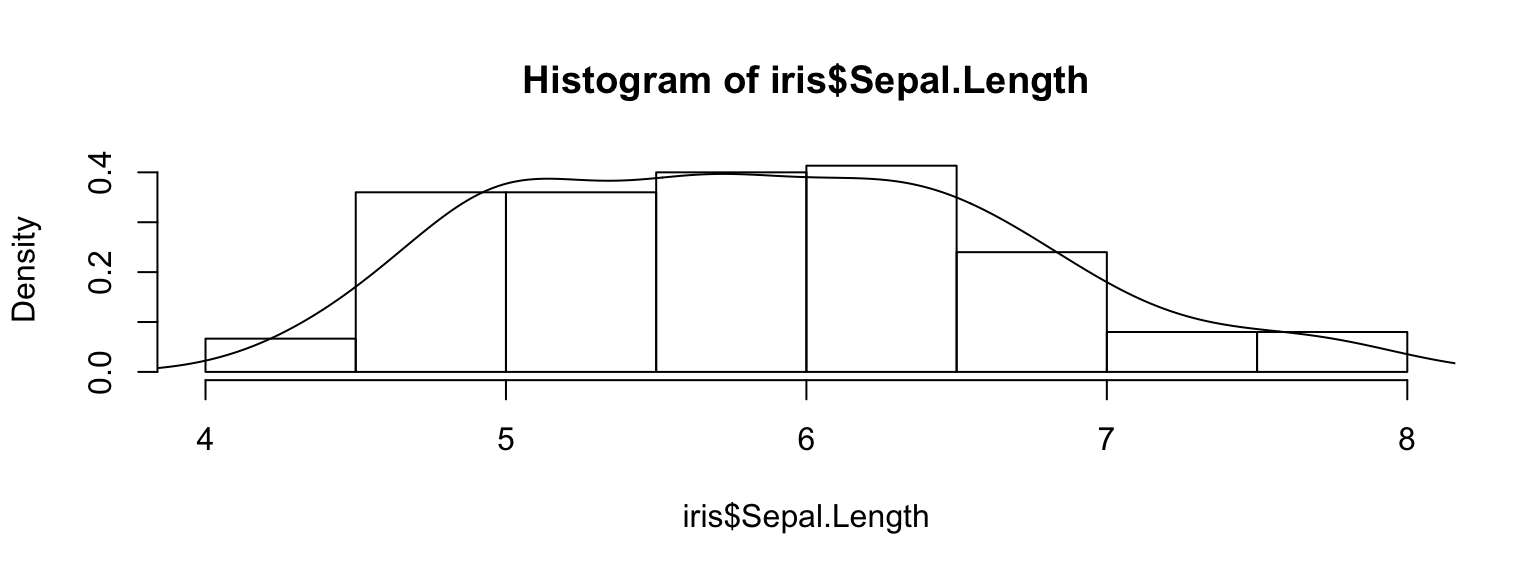
\includegraphics{Data_Mining_with_R_part_1_files/figure-beamer/unnamed-chunk-2-1.pdf}

\end{frame}

\begin{frame}[fragile]{}

Next data in categorical type

\begin{Shaded}
\begin{Highlighting}[]
\NormalTok{categories <-}\StringTok{ }\KeywordTok{table}\NormalTok{(iris$Species)}
\KeywordTok{barplot}\NormalTok{(categories, }\DataTypeTok{col =} \KeywordTok{c}\NormalTok{(}\StringTok{"red"}\NormalTok{, }\StringTok{"white"}\NormalTok{, }\StringTok{"blue"}\NormalTok{))}
\end{Highlighting}
\end{Shaded}

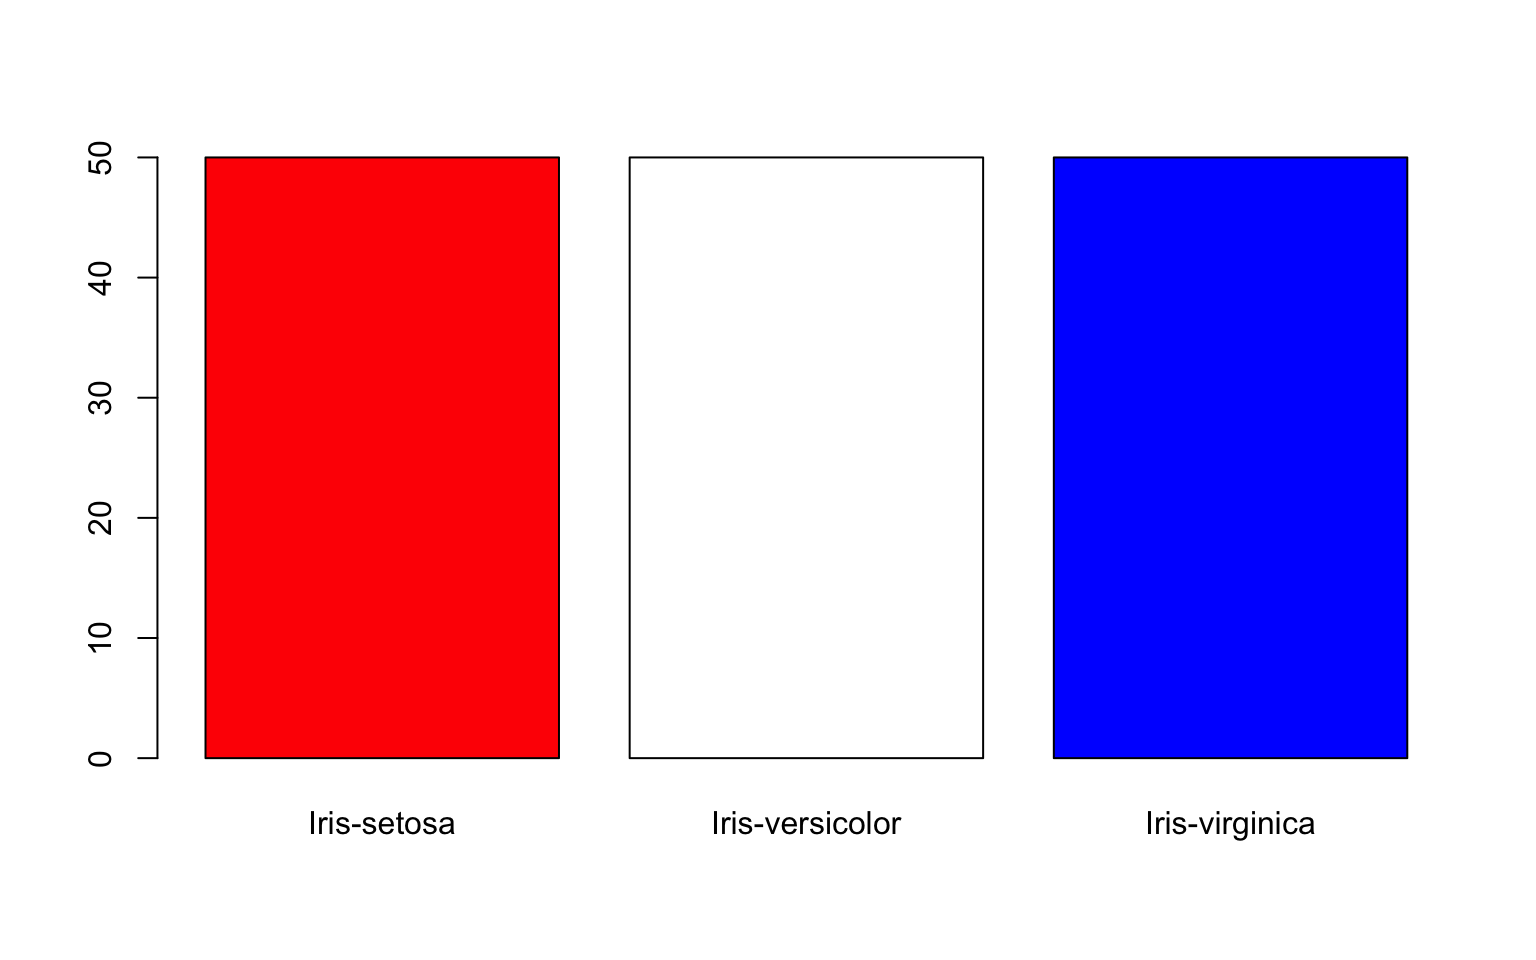
\includegraphics{Data_Mining_with_R_part_1_files/figure-beamer/unnamed-chunk-3-1.pdf}

\end{frame}

\begin{frame}[fragile]{}

Let cross data between numeric and categorical

\begin{Shaded}
\begin{Highlighting}[]
\KeywordTok{boxplot}\NormalTok{(Sepal.Length ~}\StringTok{ }\NormalTok{Species, }\DataTypeTok{data =} \NormalTok{iris, }\DataTypeTok{col =} \KeywordTok{c}\NormalTok{(}\StringTok{"pink"}\NormalTok{))}
\end{Highlighting}
\end{Shaded}

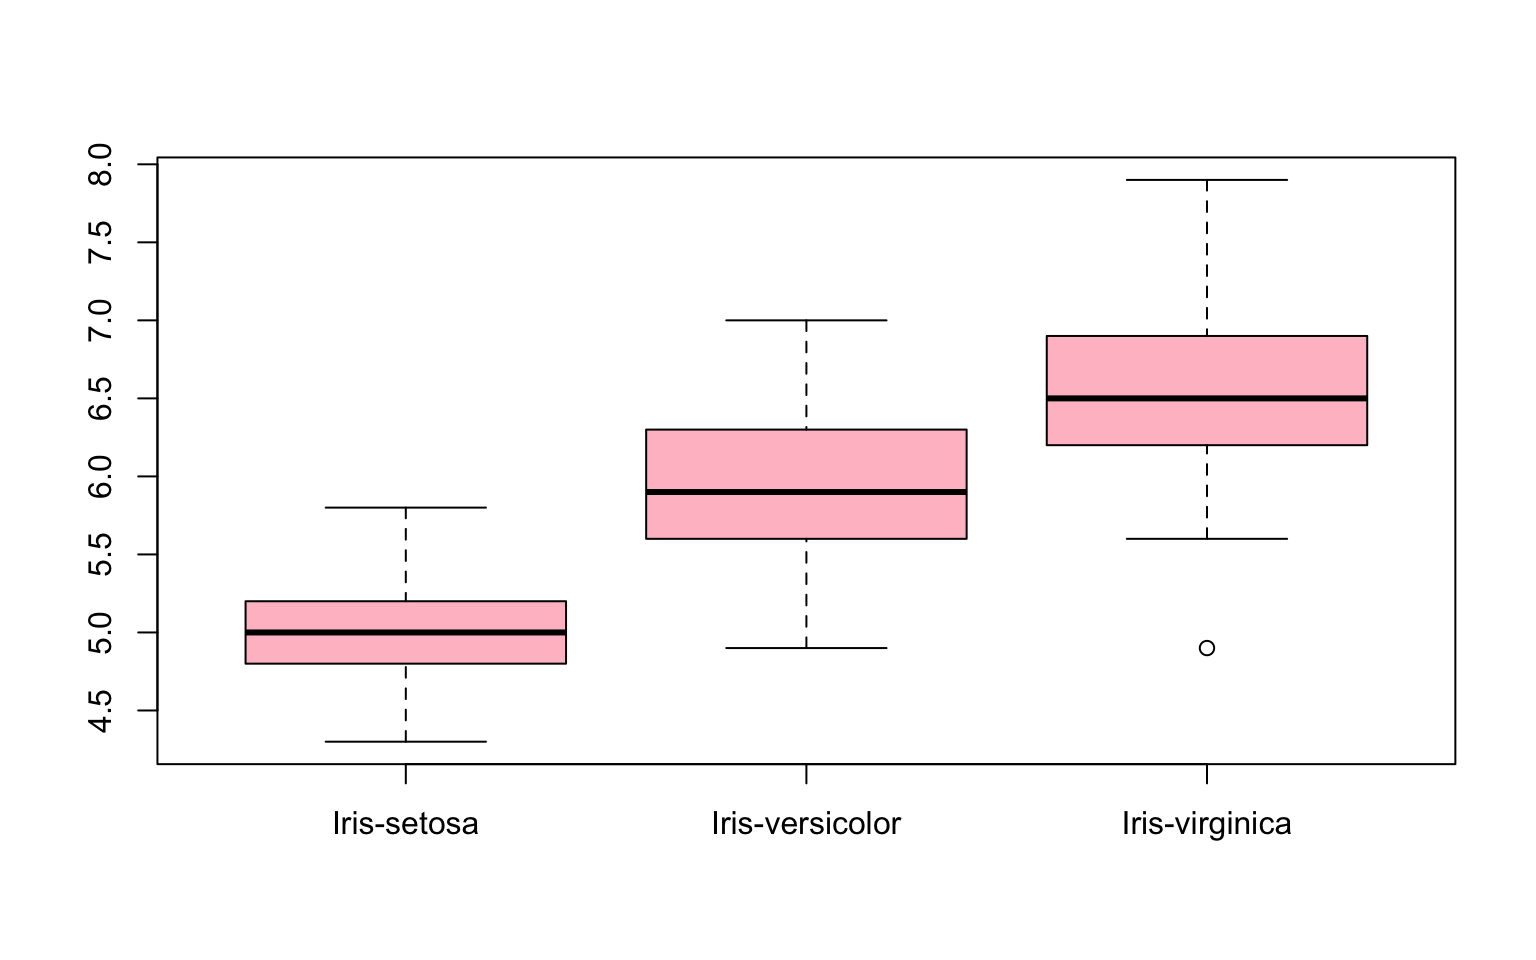
\includegraphics{Data_Mining_with_R_part_1_files/figure-beamer/unnamed-chunk-4-1.pdf}

\end{frame}

\begin{frame}[fragile]{}

Next, let do correlation in charts using ``pairs''

\begin{Shaded}
\begin{Highlighting}[]
\CommentTok{# Scatter plot for all pairs}
\KeywordTok{pairs}\NormalTok{(iris[, }\KeywordTok{c}\NormalTok{(}\DecValTok{1}\NormalTok{, }\DecValTok{2}\NormalTok{, }\DecValTok{3}\NormalTok{, }\DecValTok{4}\NormalTok{)])}
\end{Highlighting}
\end{Shaded}

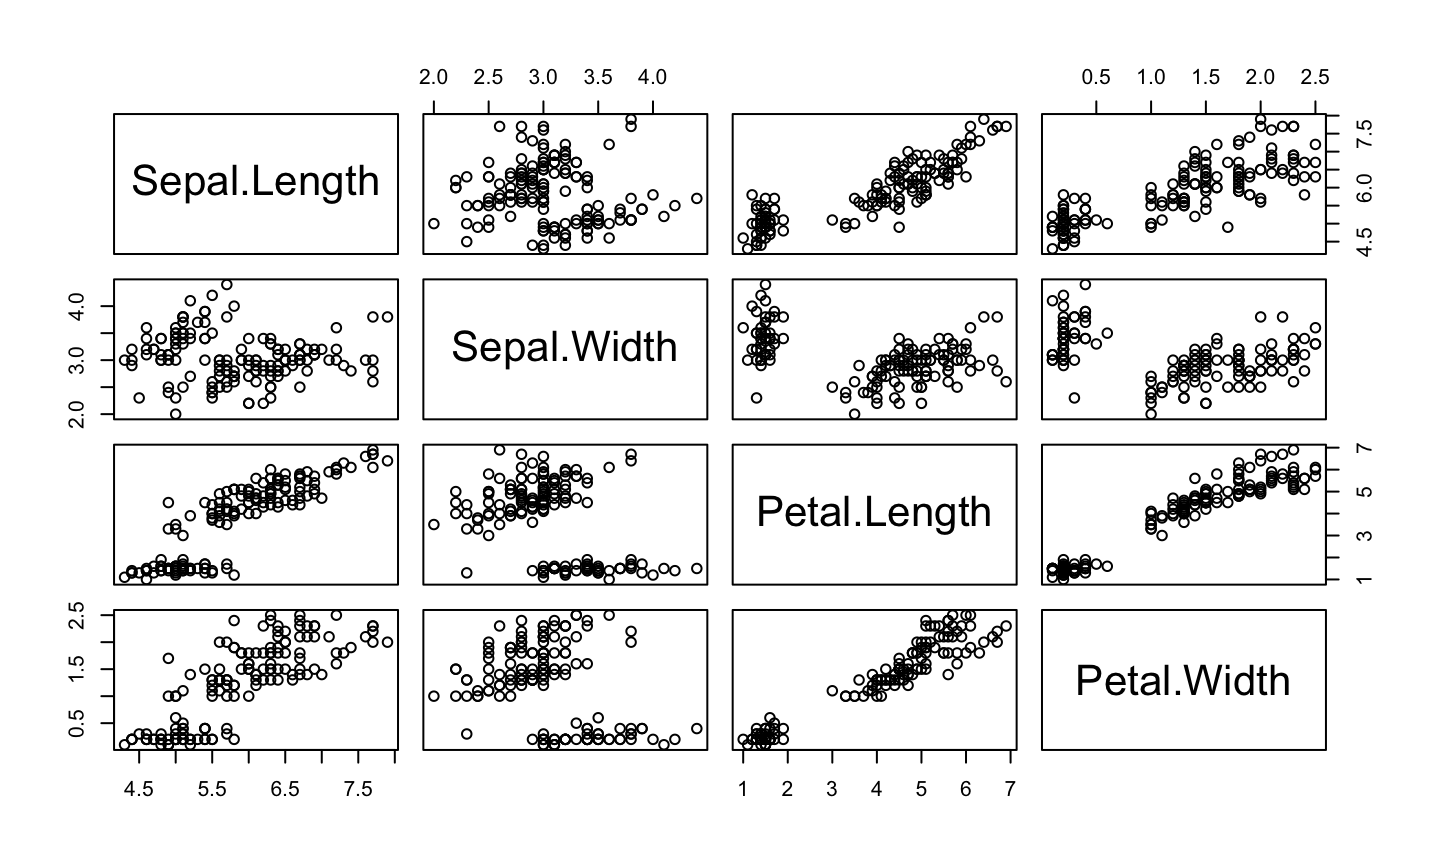
\includegraphics{Data_Mining_with_R_part_1_files/figure-beamer/unnamed-chunk-5-1.pdf}

\end{frame}

\begin{frame}[fragile]{}

Compute the correlation matrix

\begin{Shaded}
\begin{Highlighting}[]
\CommentTok{# Compute the correlation matrix}
\KeywordTok{cor}\NormalTok{(iris[, }\KeywordTok{c}\NormalTok{(}\DecValTok{1}\NormalTok{, }\DecValTok{2}\NormalTok{, }\DecValTok{3}\NormalTok{, }\DecValTok{4}\NormalTok{)])}
\end{Highlighting}
\end{Shaded}

\begin{verbatim}
##              Sepal.Length Sepal.Width Petal.Length Petal.Width
## Sepal.Length    1.0000000  -0.1093692    0.8717542   0.8179536
## Sepal.Width    -0.1093692   1.0000000   -0.4205161  -0.3565441
## Petal.Length    0.8717542  -0.4205161    1.0000000   0.9627571
## Petal.Width     0.8179536  -0.3565441    0.9627571   1.0000000
\end{verbatim}

\end{frame}

\begin{frame}[fragile]{}

Draw regression line for suspect attribute to see relationship

\begin{Shaded}
\begin{Highlighting}[]
\KeywordTok{plot}\NormalTok{(Petal.Width ~}\StringTok{ }\NormalTok{Sepal.Length, }\DataTypeTok{data =} \NormalTok{iris)}
\NormalTok{model <-}\StringTok{ }\KeywordTok{lm}\NormalTok{(Petal.Width ~}\StringTok{ }\NormalTok{Sepal.Length, }\DataTypeTok{data =} \NormalTok{iris)}
\KeywordTok{abline}\NormalTok{(model)}
\NormalTok{model2 <-}\StringTok{ }\KeywordTok{lowess}\NormalTok{(iris$Petal.Width ~}\StringTok{ }\NormalTok{iris$Sepal.Length)}
\KeywordTok{lines}\NormalTok{(model2, }\DataTypeTok{col =} \StringTok{"red"}\NormalTok{)}
\end{Highlighting}
\end{Shaded}

\includegraphics{Data_Mining_with_R_part_1_files/figure-beamer/unnamed-chunk-7-1.pdf}

\end{frame}

\begin{frame}[fragile]{Preparing Training Data}

At this step, the purpose is to transform the raw data in a form that
can fit into the data mining model.

\begin{verbatim}
- Data sampling
- Data validation and handle missing data
- Normalize numeric value into a uniform range
- Compute aggregated value (a special case is to compute frequency counts)
- Expand categorical field to binary fields
- Discretize numeric value into categories
- Create derived fields from existing fields
- Reduce dimensionality
- Power and Log transformation
\end{verbatim}

\end{frame}

\begin{frame}[fragile]{Data Sampling}

\begin{Shaded}
\begin{Highlighting}[]
\CommentTok{# Select 10 records out from iris with replacement}
\NormalTok{index <-}\StringTok{ }\KeywordTok{sample}\NormalTok{(}\DecValTok{1}\NormalTok{:}\KeywordTok{nrow}\NormalTok{(iris), }\DecValTok{10}\NormalTok{, }\DataTypeTok{replace =} \NormalTok{T)}
\NormalTok{index}
\end{Highlighting}
\end{Shaded}

\begin{verbatim}
##  [1]  23 143 150  45  32   5  82  14  94  75
\end{verbatim}

\end{frame}

\begin{frame}[fragile]{}

\begin{Shaded}
\begin{Highlighting}[]
\CommentTok{# Subset iris to irissample from index}
\NormalTok{irissample <-}\StringTok{ }\NormalTok{iris[index, ]}
\NormalTok{irissample}
\end{Highlighting}
\end{Shaded}

\begin{verbatim}
##     Sepal.Length Sepal.Width Petal.Length Petal.Width         Species
## 23           4.6         3.6          1.0         0.2     Iris-setosa
## 143          5.8         2.7          5.1         1.9  Iris-virginica
## 150          5.9         3.0          5.1         1.8  Iris-virginica
## 45           5.1         3.8          1.9         0.4     Iris-setosa
## 32           5.4         3.4          1.5         0.4     Iris-setosa
## 5            5.0         3.6          1.4         0.2     Iris-setosa
## 82           5.5         2.4          3.7         1.0 Iris-versicolor
## 14           4.3         3.0          1.1         0.1     Iris-setosa
## 94           5.0         2.3          3.3         1.0 Iris-versicolor
## 75           6.4         2.9          4.3         1.3 Iris-versicolor
\end{verbatim}

\end{frame}

\begin{frame}[fragile]{Impute missing data}

\begin{itemize}
\tightlist
\item
  Discard the whole record
\item
  Infer missing data with Average or Median
\end{itemize}

\begin{Shaded}
\begin{Highlighting}[]
\CommentTok{# Create some missing data}
\NormalTok{irissample[}\DecValTok{10}\NormalTok{, }\DecValTok{1}\NormalTok{] <-}\StringTok{ }\OtherTok{NA}
\NormalTok{irissample}
\end{Highlighting}
\end{Shaded}

\begin{verbatim}
##     Sepal.Length Sepal.Width Petal.Length Petal.Width         Species
## 23           4.6         3.6          1.0         0.2     Iris-setosa
## 143          5.8         2.7          5.1         1.9  Iris-virginica
## 150          5.9         3.0          5.1         1.8  Iris-virginica
## 45           5.1         3.8          1.9         0.4     Iris-setosa
## 32           5.4         3.4          1.5         0.4     Iris-setosa
## 5            5.0         3.6          1.4         0.2     Iris-setosa
## 82           5.5         2.4          3.7         1.0 Iris-versicolor
## 14           4.3         3.0          1.1         0.1     Iris-setosa
## 94           5.0         2.3          3.3         1.0 Iris-versicolor
## 75            NA         2.9          4.3         1.3 Iris-versicolor
\end{verbatim}

\end{frame}

\begin{frame}[fragile]{}

\begin{Shaded}
\begin{Highlighting}[]
\CommentTok{# Fix using Mean}
\KeywordTok{library}\NormalTok{(e1071)}
\NormalTok{fixiris1 <-}\StringTok{ }\KeywordTok{impute}\NormalTok{(irissample[, }\DecValTok{1}\NormalTok{:}\DecValTok{4}\NormalTok{], }\DataTypeTok{what =} \StringTok{"mean"}\NormalTok{)}
\NormalTok{fixiris1}
\end{Highlighting}
\end{Shaded}

\begin{verbatim}
##     Sepal.Length Sepal.Width Petal.Length Petal.Width
## 23      4.600000         3.6          1.0         0.2
## 143     5.800000         2.7          5.1         1.9
## 150     5.900000         3.0          5.1         1.8
## 45      5.100000         3.8          1.9         0.4
## 32      5.400000         3.4          1.5         0.4
## 5       5.000000         3.6          1.4         0.2
## 82      5.500000         2.4          3.7         1.0
## 14      4.300000         3.0          1.1         0.1
## 94      5.000000         2.3          3.3         1.0
## 75      5.177778         2.9          4.3         1.3
\end{verbatim}

\end{frame}

\begin{frame}[fragile]{}

\begin{Shaded}
\begin{Highlighting}[]
\CommentTok{# Fix using Median}
\KeywordTok{library}\NormalTok{(e1071)}
\NormalTok{fixiris2 <-}\StringTok{ }\KeywordTok{impute}\NormalTok{(irissample[, }\DecValTok{1}\NormalTok{:}\DecValTok{4}\NormalTok{], }\DataTypeTok{what =} \StringTok{"median"}\NormalTok{)}
\NormalTok{fixiris2}
\end{Highlighting}
\end{Shaded}

\begin{verbatim}
##     Sepal.Length Sepal.Width Petal.Length Petal.Width
## 23           4.6         3.6          1.0         0.2
## 143          5.8         2.7          5.1         1.9
## 150          5.9         3.0          5.1         1.8
## 45           5.1         3.8          1.9         0.4
## 32           5.4         3.4          1.5         0.4
## 5            5.0         3.6          1.4         0.2
## 82           5.5         2.4          3.7         1.0
## 14           4.3         3.0          1.1         0.1
## 94           5.0         2.3          3.3         1.0
## 75           5.1         2.9          4.3         1.3
\end{verbatim}

\end{frame}

\begin{frame}[fragile]{Normalize numeric value}

\begin{Shaded}
\begin{Highlighting}[]
\CommentTok{# Scale the colums x-mean(x)/standard deviation}
\NormalTok{scaleiris <-}\StringTok{ }\KeywordTok{scale}\NormalTok{(iris[, }\DecValTok{1}\NormalTok{:}\DecValTok{4}\NormalTok{])}
\KeywordTok{head}\NormalTok{(scaleiris)}
\end{Highlighting}
\end{Shaded}

\begin{verbatim}
##      Sepal.Length Sepal.Width Petal.Length Petal.Width
## [1,]   -0.8976739   1.0286113    -1.336794   -1.308593
## [2,]   -1.1392005  -0.1245404    -1.336794   -1.308593
## [3,]   -1.3807271   0.3367203    -1.393470   -1.308593
## [4,]   -1.5014904   0.1060900    -1.280118   -1.308593
## [5,]   -1.0184372   1.2592416    -1.336794   -1.308593
## [6,]   -0.5353840   1.9511326    -1.166767   -1.046525
\end{verbatim}

\end{frame}

\begin{frame}[fragile]{Reduce dimension}

There are two ways to reduce the number of input attributes.

\begin{verbatim}
1. Removing irrelevant input variables.
2. Removing redundant input variables.
\end{verbatim}

\end{frame}

\begin{frame}[fragile]{}

\begin{Shaded}
\begin{Highlighting}[]
\CommentTok{# Use iris data set}
\KeywordTok{cor}\NormalTok{(iris[, -}\DecValTok{5}\NormalTok{])}
\end{Highlighting}
\end{Shaded}

\begin{verbatim}
##              Sepal.Length Sepal.Width Petal.Length Petal.Width
## Sepal.Length    1.0000000  -0.1093692    0.8717542   0.8179536
## Sepal.Width    -0.1093692   1.0000000   -0.4205161  -0.3565441
## Petal.Length    0.8717542  -0.4205161    1.0000000   0.9627571
## Petal.Width     0.8179536  -0.3565441    0.9627571   1.0000000
\end{verbatim}

\begin{Shaded}
\begin{Highlighting}[]
\CommentTok{# Compute PCA Notice that PC1 and PC2 covers most variation}
\NormalTok{pca <-}\StringTok{ }\KeywordTok{prcomp}\NormalTok{(iris[, -}\DecValTok{5}\NormalTok{], }\DataTypeTok{scale =} \NormalTok{T)}
\KeywordTok{summary}\NormalTok{(pca)}
\end{Highlighting}
\end{Shaded}

\begin{verbatim}
## Importance of components:
##                           PC1    PC2     PC3     PC4
## Standard deviation     1.7061 0.9598 0.38387 0.14355
## Proportion of Variance 0.7277 0.2303 0.03684 0.00515
## Cumulative Proportion  0.7277 0.9580 0.99485 1.00000
\end{verbatim}

\end{frame}

\begin{frame}[fragile]{}

\begin{Shaded}
\begin{Highlighting}[]
\CommentTok{# Plot PCA}
\KeywordTok{plot}\NormalTok{(pca)}
\end{Highlighting}
\end{Shaded}

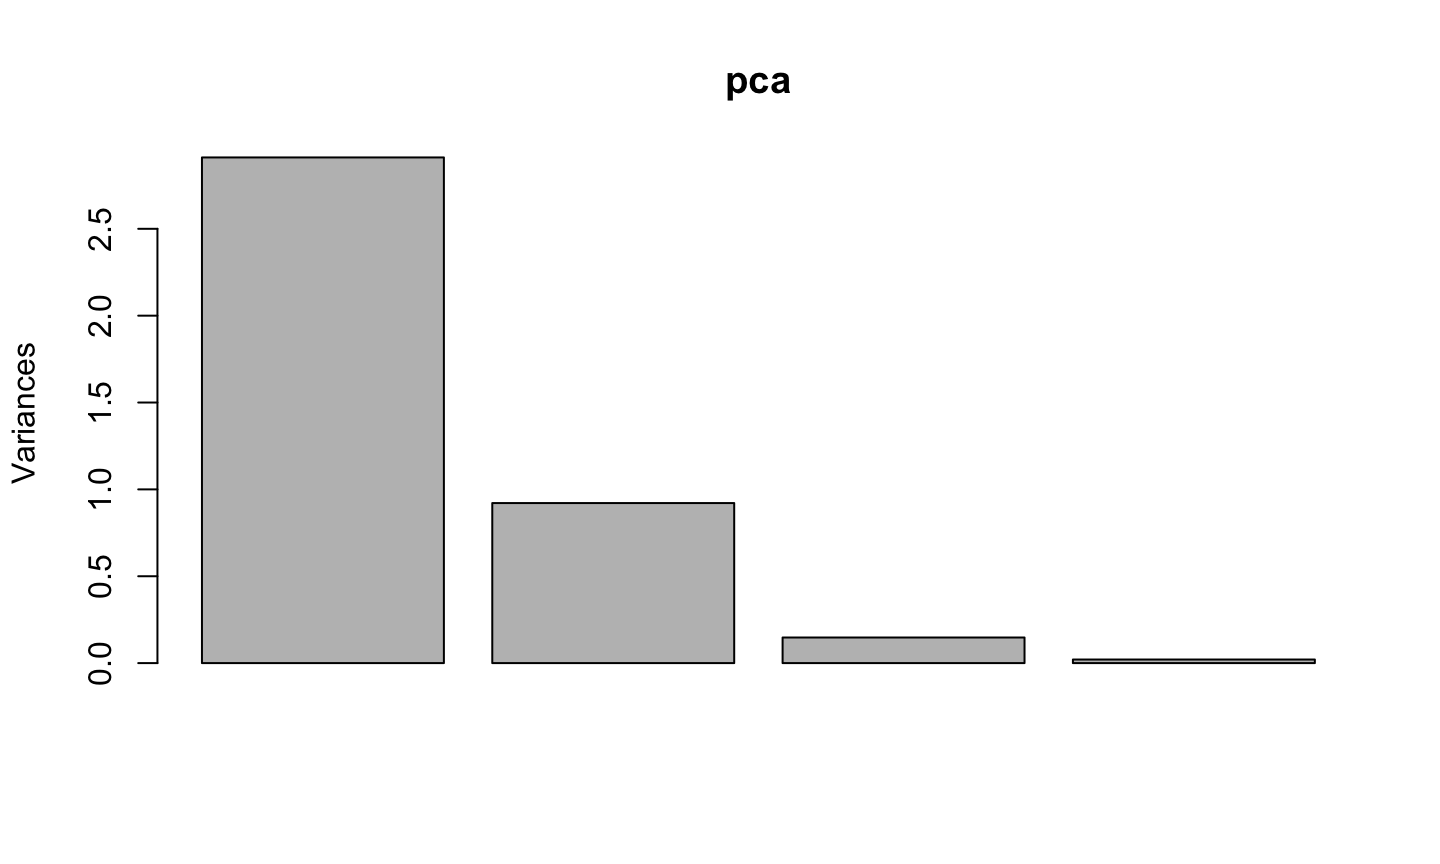
\includegraphics{Data_Mining_with_R_part_1_files/figure-beamer/unnamed-chunk-15-1.pdf}

\end{frame}

\begin{frame}[fragile]{}

\begin{Shaded}
\begin{Highlighting}[]
\NormalTok{pca$rotation}
\end{Highlighting}
\end{Shaded}

\begin{verbatim}
##                     PC1         PC2        PC3        PC4
## Sepal.Length  0.5223716 -0.37231836  0.7210168  0.2619956
## Sepal.Width  -0.2633549 -0.92555649 -0.2420329 -0.1241348
## Petal.Length  0.5812540 -0.02109478 -0.1408923 -0.8011543
## Petal.Width   0.5656110 -0.06541577 -0.6338014  0.5235463
\end{verbatim}

\end{frame}

\begin{frame}[fragile]{}

\begin{Shaded}
\begin{Highlighting}[]
\KeywordTok{predict}\NormalTok{(pca)[}\DecValTok{1}\NormalTok{:}\DecValTok{2}\NormalTok{, ]}
\end{Highlighting}
\end{Shaded}

\begin{verbatim}
##            PC1        PC2       PC3        PC4
## [1,] -2.256981 -0.5040154 0.1215362 0.02299628
## [2,] -2.079459  0.6532164 0.2264921 0.10286364
\end{verbatim}

\begin{Shaded}
\begin{Highlighting}[]
\KeywordTok{biplot}\NormalTok{(pca)}
\end{Highlighting}
\end{Shaded}

\includegraphics{Data_Mining_with_R_part_1_files/figure-beamer/unnamed-chunk-17-1.pdf}

\end{frame}

\begin{frame}[fragile]{Add derived attributes}

\begin{Shaded}
\begin{Highlighting}[]
\NormalTok{iris2 <-}\StringTok{ }\KeywordTok{transform}\NormalTok{(iris, }\DataTypeTok{ratio =} \KeywordTok{round}\NormalTok{(Sepal.Length/Sepal.Width, }
    \DecValTok{2}\NormalTok{))}
\KeywordTok{head}\NormalTok{(iris2)}
\end{Highlighting}
\end{Shaded}

\begin{verbatim}
##   Sepal.Length Sepal.Width Petal.Length Petal.Width     Species ratio
## 1          5.1         3.5          1.4         0.2 Iris-setosa  1.46
## 2          4.9         3.0          1.4         0.2 Iris-setosa  1.63
## 3          4.7         3.2          1.3         0.2 Iris-setosa  1.47
## 4          4.6         3.1          1.5         0.2 Iris-setosa  1.48
## 5          5.0         3.6          1.4         0.2 Iris-setosa  1.39
## 6          5.4         3.9          1.7         0.4 Iris-setosa  1.38
\end{verbatim}

\end{frame}

\begin{frame}[fragile]{Discretize numeric value into categories}

\begin{Shaded}
\begin{Highlighting}[]
\CommentTok{# Equal width cuts}
\NormalTok{segments =}\StringTok{ }\DecValTok{10}
\NormalTok{maxL <-}\StringTok{ }\KeywordTok{max}\NormalTok{(iris$Petal.Length)}
\NormalTok{minL <-}\StringTok{ }\KeywordTok{min}\NormalTok{(iris$Petal.Length)}
\NormalTok{theBreaks <-}\StringTok{ }\KeywordTok{seq}\NormalTok{(minL, maxL, }\DataTypeTok{by =} \NormalTok{(maxL -}\StringTok{ }\NormalTok{minL)/segments)}
\NormalTok{cutPetalLength <-}\StringTok{ }\KeywordTok{cut}\NormalTok{(iris$Petal.Length, }\DataTypeTok{breaks =} \NormalTok{theBreaks, }
    \DataTypeTok{include.lowest =} \NormalTok{T)}
\NormalTok{newdata <-}\StringTok{ }\KeywordTok{data.frame}\NormalTok{(}\DataTypeTok{origin.Petal.Len =} \NormalTok{iris$Petal.Length, }
    \DataTypeTok{cut.Petal.Len =} \NormalTok{cutPetalLength)}
\KeywordTok{head}\NormalTok{(newdata)}
\end{Highlighting}
\end{Shaded}

\begin{verbatim}
##   origin.Petal.Len cut.Petal.Len
## 1              1.4      [1,1.59]
## 2              1.4      [1,1.59]
## 3              1.3      [1,1.59]
## 4              1.5      [1,1.59]
## 5              1.4      [1,1.59]
## 6              1.7   (1.59,2.18]
\end{verbatim}

\end{frame}

\begin{frame}[fragile]{}

\begin{Shaded}
\begin{Highlighting}[]
\CommentTok{# Constant frequency / height}
\NormalTok{myBreaks <-}\StringTok{ }\KeywordTok{quantile}\NormalTok{(iris$Petal.Length, }\DataTypeTok{probs =} \KeywordTok{seq}\NormalTok{(}\DecValTok{0}\NormalTok{, }\DecValTok{1}\NormalTok{, }\DecValTok{1}\NormalTok{/segments))}
\NormalTok{cutPetalLength2 <-}\StringTok{ }\KeywordTok{cut}\NormalTok{(iris$Petal.Length, }\DataTypeTok{breaks =} \NormalTok{myBreaks, }
    \DataTypeTok{include.lowest =} \NormalTok{T)}
\NormalTok{newdata2 <-}\StringTok{ }\KeywordTok{data.frame}\NormalTok{(}\DataTypeTok{orig.Petal.Lens =} \NormalTok{iris$Petal.Length, }
    \DataTypeTok{cut.Petal.Len =} \NormalTok{cutPetalLength2)}
\KeywordTok{head}\NormalTok{(newdata2)}
\end{Highlighting}
\end{Shaded}

\begin{verbatim}
##   orig.Petal.Lens cut.Petal.Len
## 1             1.4       [1,1.4]
## 2             1.4       [1,1.4]
## 3             1.3       [1,1.4]
## 4             1.5     (1.4,1.5]
## 5             1.4       [1,1.4]
## 6             1.7     (1.7,3.9]
\end{verbatim}

\end{frame}

\begin{frame}[fragile]{Binarize categorical attributes}

\begin{Shaded}
\begin{Highlighting}[]
\NormalTok{cat <-}\StringTok{ }\KeywordTok{levels}\NormalTok{(iris$Species)}
\NormalTok{binarize <-}\StringTok{ }\NormalTok{function(x) \{}
    \KeywordTok{return}\NormalTok{(iris$Species ==}\StringTok{ }\NormalTok{x)}
\NormalTok{\}}
\NormalTok{newcols <-}\StringTok{ }\KeywordTok{sapply}\NormalTok{(cat, binarize)}
\KeywordTok{colnames}\NormalTok{(newcols) <-}\StringTok{ }\NormalTok{cat}
\NormalTok{data <-}\StringTok{ }\KeywordTok{cbind}\NormalTok{(iris[, }\KeywordTok{c}\NormalTok{(}\StringTok{"Species"}\NormalTok{)], newcols)}
\end{Highlighting}
\end{Shaded}

\end{frame}

\begin{frame}[fragile]{Binarize categorical attributes (cont)}

\begin{Shaded}
\begin{Highlighting}[]
\NormalTok{data[}\DecValTok{45}\NormalTok{:}\DecValTok{55}\NormalTok{, ]}
\end{Highlighting}
\end{Shaded}

\begin{verbatim}
##         Iris-setosa Iris-versicolor Iris-virginica
##  [1,] 1           1               0              0
##  [2,] 1           1               0              0
##  [3,] 1           1               0              0
##  [4,] 1           1               0              0
##  [5,] 1           1               0              0
##  [6,] 1           1               0              0
##  [7,] 2           0               1              0
##  [8,] 2           0               1              0
##  [9,] 2           0               1              0
## [10,] 2           0               1              0
## [11,] 2           0               1              0
\end{verbatim}

\end{frame}

\section{Data Mining Techniques}\label{data-mining-techniques}

\begin{frame}[fragile]{Iris Data Preparation}

\begin{Shaded}
\begin{Highlighting}[]
\CommentTok{# sample iris into 2 sets (training, testing) with 70%/30%}
\KeywordTok{set.seed}\NormalTok{(}\DecValTok{1234}\NormalTok{)}
\NormalTok{ind <-}\StringTok{ }\KeywordTok{sample}\NormalTok{(}\DecValTok{2}\NormalTok{, }\KeywordTok{nrow}\NormalTok{(iris), }\DataTypeTok{replace =} \OtherTok{TRUE}\NormalTok{, }\DataTypeTok{prob =} \KeywordTok{c}\NormalTok{(}\FloatTok{0.7}\NormalTok{, }
    \FloatTok{0.3}\NormalTok{))}
\NormalTok{trainData <-}\StringTok{ }\NormalTok{iris[ind ==}\StringTok{ }\DecValTok{1}\NormalTok{, ]}
\NormalTok{testData <-}\StringTok{ }\NormalTok{iris[ind ==}\StringTok{ }\DecValTok{2}\NormalTok{, ]}
\end{Highlighting}
\end{Shaded}

\end{frame}

\begin{frame}{Decision Tree}

Libray name -\textgreater{} party

Function name -\textgreater{} ctree

Installation

install.packages(``party'')

\end{frame}

\begin{frame}[fragile]{Decision Tree - Create Model}

\begin{Shaded}
\begin{Highlighting}[]
\KeywordTok{library}\NormalTok{(party)}
\NormalTok{myFormula <-}\StringTok{ }\NormalTok{Species ~}\StringTok{ }\NormalTok{Sepal.Length +}\StringTok{ }\NormalTok{Sepal.Width +}\StringTok{ }\NormalTok{Petal.Length +}\StringTok{ }
\StringTok{    }\NormalTok{Petal.Width}
\NormalTok{iris_ctree <-}\StringTok{ }\KeywordTok{ctree}\NormalTok{(myFormula, }\DataTypeTok{data =} \NormalTok{trainData)}
\CommentTok{# Check the prediction}
\KeywordTok{table}\NormalTok{(}\KeywordTok{predict}\NormalTok{(iris_ctree), trainData$Species)}
\end{Highlighting}
\end{Shaded}

\begin{verbatim}
##                  
##                   Iris-setosa Iris-versicolor Iris-virginica
##   Iris-setosa              40               0              0
##   Iris-versicolor           0              37              3
##   Iris-virginica            0               1             31
\end{verbatim}

\end{frame}

\begin{frame}[fragile]{}

\begin{Shaded}
\begin{Highlighting}[]
\KeywordTok{print}\NormalTok{(iris_ctree)}
\end{Highlighting}
\end{Shaded}

\begin{verbatim}
## 
##   Conditional inference tree with 4 terminal nodes
## 
## Response:  Species 
## Inputs:  Sepal.Length, Sepal.Width, Petal.Length, Petal.Width 
## Number of observations:  112 
## 
## 1) Petal.Length <= 1.9; criterion = 1, statistic = 104.637
##   2)*  weights = 40 
## 1) Petal.Length > 1.9
##   3) Petal.Width <= 1.7; criterion = 1, statistic = 48.939
##     4) Petal.Length <= 4.4; criterion = 0.974, statistic = 7.397
##       5)*  weights = 21 
##     4) Petal.Length > 4.4
##       6)*  weights = 19 
##   3) Petal.Width > 1.7
##     7)*  weights = 32
\end{verbatim}

\end{frame}

\begin{frame}[fragile]{}

\begin{Shaded}
\begin{Highlighting}[]
\KeywordTok{plot}\NormalTok{(iris_ctree)}
\end{Highlighting}
\end{Shaded}

\includegraphics{Data_Mining_with_R_part_1_files/figure-beamer/unnamed-chunk-26-1.pdf}

\end{frame}

\begin{frame}[fragile]{}

\begin{Shaded}
\begin{Highlighting}[]
\KeywordTok{plot}\NormalTok{(iris_ctree, }\DataTypeTok{type =} \StringTok{"simple"}\NormalTok{)}
\end{Highlighting}
\end{Shaded}

\includegraphics{Data_Mining_with_R_part_1_files/figure-beamer/unnamed-chunk-27-1.pdf}

\end{frame}

\begin{frame}[fragile]{Decision Tree - Prediction}

\begin{Shaded}
\begin{Highlighting}[]
\CommentTok{# Predict on test data}
\NormalTok{testPred <-}\StringTok{ }\KeywordTok{predict}\NormalTok{(iris_ctree, }\DataTypeTok{newdata =} \NormalTok{testData)}
\KeywordTok{table}\NormalTok{(testPred, testData$Species)}
\end{Highlighting}
\end{Shaded}

\begin{verbatim}
##                  
## testPred          Iris-setosa Iris-versicolor Iris-virginica
##   Iris-setosa              10               0              0
##   Iris-versicolor           0              12              2
##   Iris-virginica            0               0             14
\end{verbatim}

\end{frame}

\begin{frame}{K-Nearest Neighbor Classfication (k-NN)}

Library -\textgreater{} class

Function -\textgreater{} knn

Installation

install.packages(``class'')

\end{frame}

\begin{frame}[fragile]{K-NN}

\begin{Shaded}
\begin{Highlighting}[]
\KeywordTok{library}\NormalTok{(class)}
\NormalTok{train_input <-}\StringTok{ }\KeywordTok{as.matrix}\NormalTok{(trainData[, -}\DecValTok{5}\NormalTok{])}
\NormalTok{train_output <-}\StringTok{ }\KeywordTok{as.vector}\NormalTok{(trainData[, }\DecValTok{5}\NormalTok{])}
\NormalTok{test_input <-}\StringTok{ }\KeywordTok{as.matrix}\NormalTok{(testData[, -}\DecValTok{5}\NormalTok{])}
\NormalTok{prediction <-}\StringTok{ }\KeywordTok{knn}\NormalTok{(train_input, test_input, train_output, }\DataTypeTok{k =} \DecValTok{5}\NormalTok{)}
\KeywordTok{table}\NormalTok{(prediction, testData$Species)}
\end{Highlighting}
\end{Shaded}

\begin{verbatim}
##                  
## prediction        Iris-setosa Iris-versicolor Iris-virginica
##   Iris-setosa              10               0              0
##   Iris-versicolor           0              12              0
##   Iris-virginica            0               0             16
\end{verbatim}

\end{frame}

\begin{frame}{Naive Bayes Classifier}

Library --\textgreater{} e1071

Function --\textgreater{} naiveBayes

Installation

install.packages(``e1071'')

\end{frame}

\begin{frame}[fragile]{Naive Bayes}

\begin{Shaded}
\begin{Highlighting}[]
\KeywordTok{library}\NormalTok{(e1071)}
\CommentTok{# can handle both categorical and numeric input but output}
\CommentTok{# must be categorical}
\NormalTok{model <-}\StringTok{ }\KeywordTok{naiveBayes}\NormalTok{(Species ~}\StringTok{ }\NormalTok{., }\DataTypeTok{data =} \NormalTok{trainData)}
\NormalTok{prediction <-}\StringTok{ }\KeywordTok{predict}\NormalTok{(model, testData[, -}\DecValTok{5}\NormalTok{])}
\KeywordTok{table}\NormalTok{(prediction, testData[, }\DecValTok{5}\NormalTok{])}
\end{Highlighting}
\end{Shaded}

\begin{verbatim}
##                  
## prediction        Iris-setosa Iris-versicolor Iris-virginica
##   Iris-setosa              10               0              0
##   Iris-versicolor           0              12              2
##   Iris-virginica            0               0             14
\end{verbatim}

\end{frame}

\begin{frame}{Neural Network}

Library --\textgreater{} neuralnet

Function --\textgreater{} neuralnet

Installation

install.packages(`neuralnet')

\end{frame}

\begin{frame}[fragile]{Neural Network}

\begin{Shaded}
\begin{Highlighting}[]
\KeywordTok{library}\NormalTok{(neuralnet)}
\NormalTok{nnet_trainData <-}\StringTok{ }\NormalTok{trainData}
\CommentTok{# Binarize the categorical output}
\NormalTok{nnet_trainData <-}\StringTok{ }\KeywordTok{cbind}\NormalTok{(nnet_trainData, trainData$Species ==}\StringTok{ }
\StringTok{    "Iris-setosa"}\NormalTok{)}
\NormalTok{nnet_trainData <-}\StringTok{ }\KeywordTok{cbind}\NormalTok{(nnet_trainData, trainData$Species ==}\StringTok{ }
\StringTok{    "Iris-versicolor"}\NormalTok{)}
\NormalTok{nnet_trainData <-}\StringTok{ }\KeywordTok{cbind}\NormalTok{(nnet_trainData, trainData$Species ==}\StringTok{ }
\StringTok{    "Iris-virginica"}\NormalTok{)}
\KeywordTok{names}\NormalTok{(nnet_trainData)[}\DecValTok{6}\NormalTok{] <-}\StringTok{ "setosa"}
\KeywordTok{names}\NormalTok{(nnet_trainData)[}\DecValTok{7}\NormalTok{] <-}\StringTok{ "versicolor"}
\KeywordTok{names}\NormalTok{(nnet_trainData)[}\DecValTok{8}\NormalTok{] <-}\StringTok{ "virginica"}
\NormalTok{nn <-}\StringTok{ }\KeywordTok{neuralnet}\NormalTok{(setosa +}\StringTok{ }\NormalTok{versicolor +}\StringTok{ }\NormalTok{virginica ~}\StringTok{ }\NormalTok{Sepal.Length +}\StringTok{ }
\StringTok{    }\NormalTok{Sepal.Width +}\StringTok{ }\NormalTok{Petal.Length +}\StringTok{ }\NormalTok{Petal.Width, }\DataTypeTok{data =} \NormalTok{nnet_trainData, }
    \DataTypeTok{hidden =} \KeywordTok{c}\NormalTok{(}\DecValTok{3}\NormalTok{))}
\end{Highlighting}
\end{Shaded}

\end{frame}

\begin{frame}[fragile]{Neural Network - Plot Model}

\begin{Shaded}
\begin{Highlighting}[]
\KeywordTok{plot}\NormalTok{(nn)}
\end{Highlighting}
\end{Shaded}

\begin{figure}[htbp]
\centering
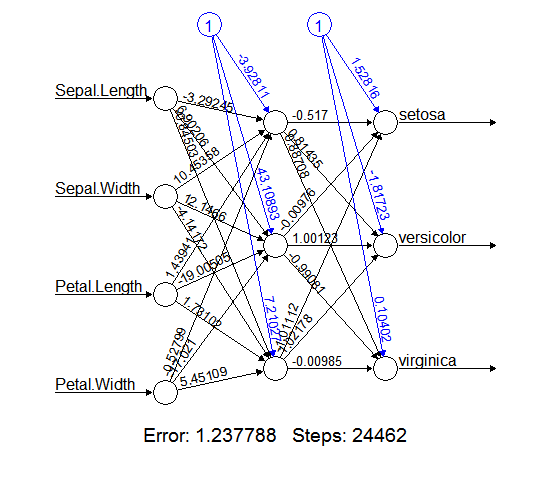
\includegraphics{nn.png}
\caption{nn}
\end{figure}

\end{frame}

\begin{frame}[fragile]{Neural Network - Prediction}

\begin{Shaded}
\begin{Highlighting}[]
\NormalTok{mypredict <-}\StringTok{ }\KeywordTok{compute}\NormalTok{(nn, testData[-}\DecValTok{5}\NormalTok{])$net.result}
\CommentTok{# put multiple binary output to categorical output}
\NormalTok{maxidx <-}\StringTok{ }\NormalTok{function(arr) \{}
    \KeywordTok{return}\NormalTok{(}\KeywordTok{which}\NormalTok{(arr ==}\StringTok{ }\KeywordTok{max}\NormalTok{(arr)))}
\NormalTok{\}}
\NormalTok{idx <-}\StringTok{ }\KeywordTok{apply}\NormalTok{(mypredict, }\KeywordTok{c}\NormalTok{(}\DecValTok{1}\NormalTok{), maxidx)}
\NormalTok{prediction <-}\StringTok{ }\KeywordTok{c}\NormalTok{(}\StringTok{"Iris-setosa"}\NormalTok{, }\StringTok{"Iris-versicolor"}\NormalTok{, }\StringTok{"Iris-virginica"}\NormalTok{)[idx]}
\KeywordTok{table}\NormalTok{(prediction, testData$Species)}
\end{Highlighting}
\end{Shaded}

\begin{verbatim}
##                  
## prediction        Iris-setosa Iris-versicolor Iris-virginica
##   Iris-setosa              10               0              0
##   Iris-versicolor           0              12              0
##   Iris-virginica            0               0             16
\end{verbatim}

\end{frame}

\section{End of Part 1}\label{end-of-part-1}

\end{document}
